\chapter{Introduction}

In this chapter I will simply introduce the subject of this master thesis, showing some basic concepts and key aspects related to it.

\section{INGInious}

INGInious is a web platform developed by the UCL.  It is a tool for automatic correction of programs written by students. To check the validity of a student's code, the latest will be executed, fed with some inputs, and the outputs generated will be checked. It currently relies on Docker containers to provide a good isolation between the machine hosting the site and the execution of the student's codes.  This allows to avoid that a problem in a program submitted by a student could have any impact on the platform.  Docker also allows to manage the resources granted to each code execution.  For now, INGInious can meet the demand and provide honest performances and responsiveness.  But looking at the growing usage of the platform, we might soon come to a point where we reach the limits of the current implementation.

\subsection{Architecture}
INGInious counts four main components:
\begin{enumerate}
  \item The front-end: the website with which each student interacts when submitting a task.
  \item The back-end: a queue of all the tasks that need to be graded.
  \item The docker agent: responsible for the container assignment to the pending tasks when resources are available.
  \item The docker containers: one for the student code and one for the teacher tests evaluating the student's code behaviour.
\end{enumerate}
The journey of a task submitted on INGInious is represented on Figure \ref{fig:architecture}.
\begin{figure}[!h]
  \begin{center}
    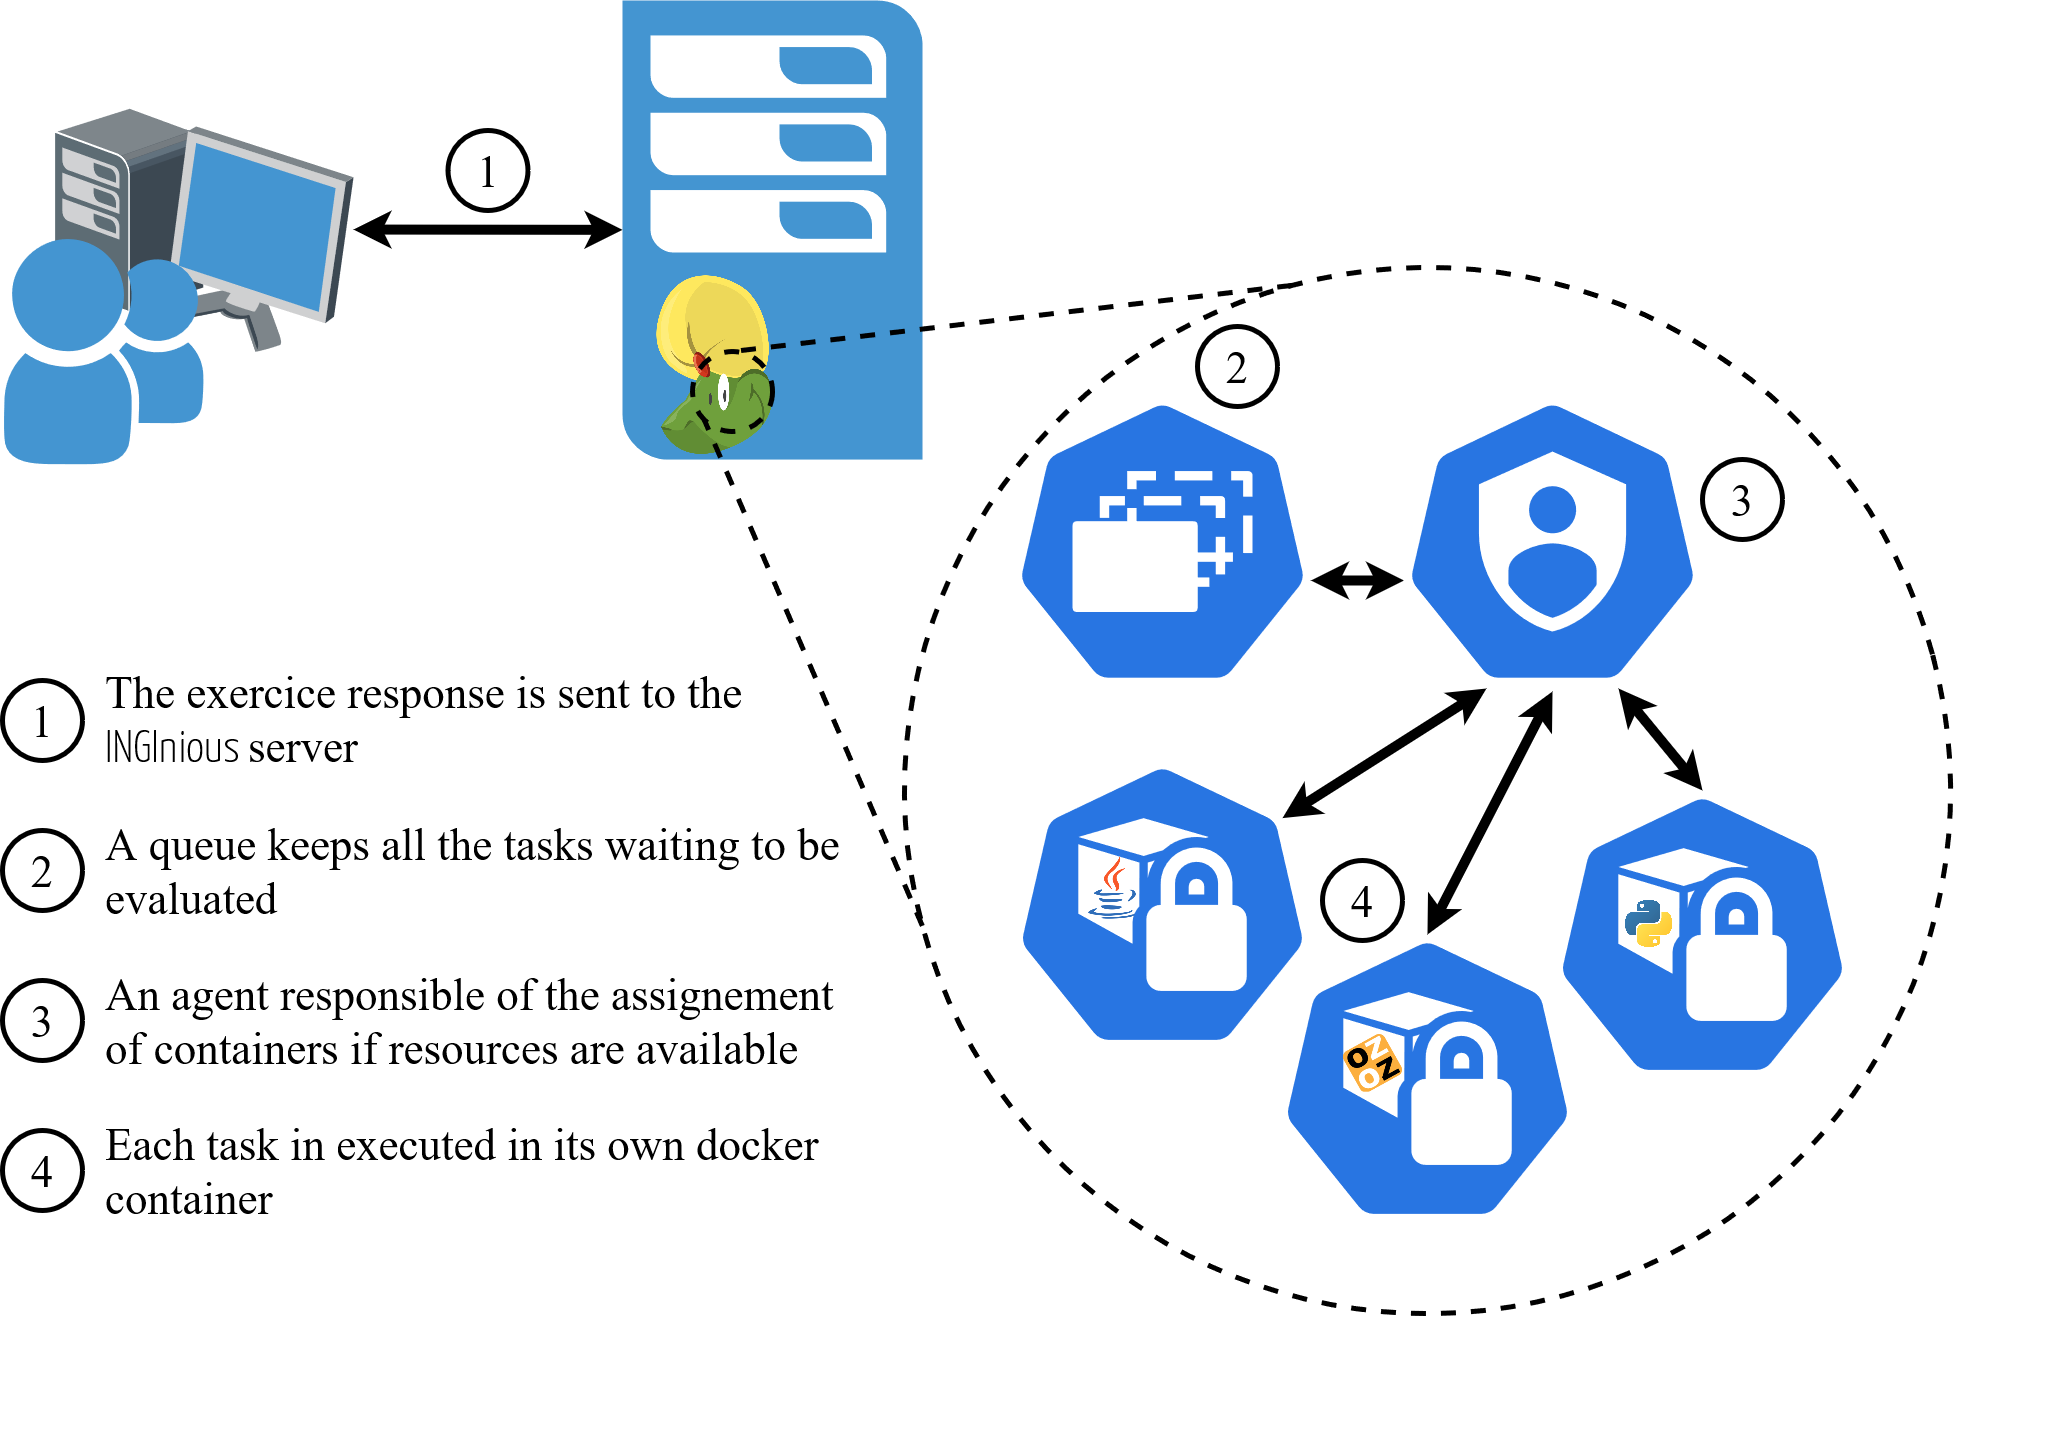
\includegraphics[width=\linewidth]{images/Architecture.png}
    \caption{INGInious global architecture}
    \label{fig:architecture}
  \end{center}
\end{figure}

\subsection{Key features}
The key features of INGInious, that allows it to meet the requirement of a code grading platform, are the following:
\begin{itemize}
  \item Isolation between the student's code and the platform.
  \item Resource limitation (CPU, RAM, Network, Pids) for the student's code execution.
  \item Modularity and versatility regarding the tasks that INGInious can correct.  Multiple programming language are supported, and new ones can easily be added.
\end{itemize}

\subsection{Bottlenecks}
When a task is submitted, we count five delays before the answer can be delivered to the student:
\begin{itemize}
  \item The sending time: the time it takes for the task to be sent to the back-end.
  \item The waiting time: the time the task will spend in the queue, waiting for an available container.
  \item The booting time: the time it takes to the container to boot and be ready to evaluate the task.
  \item The grading time: the time it takes for the code to run and for the teacher's container to grade it.
  \item The response time: the time to send the response back to the student.
\end{itemize}
For the first and the last one, supposing that the machine hosting the website is not overwhelmed, the delay depends entirely on the network. It is a bit out of our hands.  The waiting time is directly related to the current load on the platform. This is more a symptom of the server overwhelming than its cause, it could be directly solved by using a scaling strategy (see section \ref{section:scaling}).  And then we come to the booting time and the grading time, which directly depends on the containerization technology used and on the hardware performances, this is were we are going to try to see if we can improve things in this thesis.

\section{Scaling} \label{section:scaling}
Currently, the resources provided to INGInious vary, depending on the load that the platform is expected to be facing.  Typically, when the grading of an exam is done by INGInious, the platform is scaled up, and during the holidays it is scaled down.  When it comes to scaling, two strategies can be used; vertical scaling and horizontal scaling.

\paragraph{} \textbf{Vertical scaling} consists in adding more resources on a single machine, to improve its performances when needed.  For example, when the number of tasks arriving to the server grows, we could increase the number of virtual Cores allocated to the Virtual Machine (VM) hosting the platform in order to be able to threat more of them concurrently.  If the size of the waiting queue is increasing, we might want to make more RAM available.

\paragraph{} \textbf{Horizontal scaling} consists in sharing the workload across multiple machines, so that each machine can handle a small part of it.  This is a solution widely used nowadays as it allows to scale up virtually indefinitely, which is not the case with vertical scally where we depend on the maximum capacity of the hardware.  This requires rethinking the architecture of the platform globally.

\section{Intentions}
This master thesis aims at improving INGInious, regarding its performances and its scalability.  To do so, I will search and compare different containerization technologies and configurations that could be used instead of Docker's current configuration.  The goal is to find if an alternative could decrease the booting time (and the grading time) without losing any of the key features of the platform.  If such an alternative is found and proven to be worth the change, INGInious could then be refreshed with it.

Based on my research, I will answer to those three main questions:
\begin{enumerate}
  \item Compared to other available solutions, how good is the current configuration chosen by INGInious to face the responsiveness challenge of the platform?  How much better could it be?  How easy would it be to improve it?  Do some solutions involve tradeoffs in terms of maturity, support or maintainability?
  \item Could there be a solution tailor-made for the specific case of INGInious?  What would it be?  What would it cost to use it?
  \item What would be the cost of providing a stronger/safer isolation to the containers used by INGInious?  Which opportunities could it bring?
\end{enumerate}
